%\begin{figure}[hbt]
%  \centering
%  \label{fig:}
%  \subfigure[CAP]{
%    \includegraphics[width=0.4\textwidth]{}
%  }
%  \caption{}
%\end{figure}

\vspace*{\fill}

\begin{figure}[hbt]
  \centering
  \label{fig:rect}
  \subfigure[Rectangle]{
    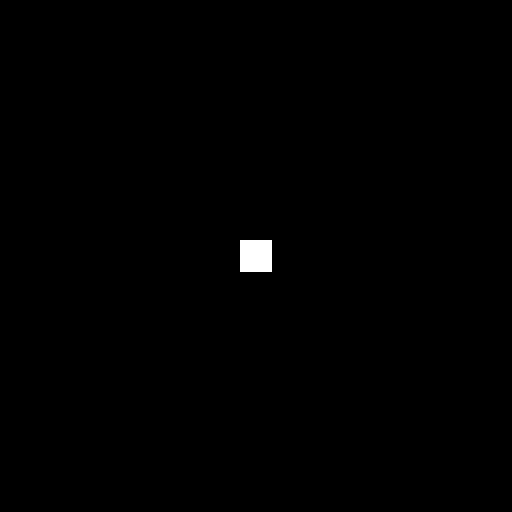
\includegraphics[width=146pt]{../images/rect}
  }
  \subfigure[Rectangle FFT]{
    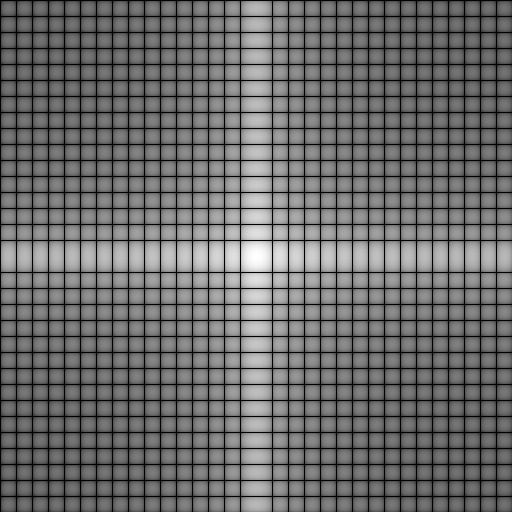
\includegraphics[width=146pt]{../images/rect_fft}
  }
  \caption{32x32 Rectangle with FFT.}
\end{figure}

\begin{figure}[hbt]
  \centering
  \label{fig:boy_fft}
  \subfigure[Original Image]{
    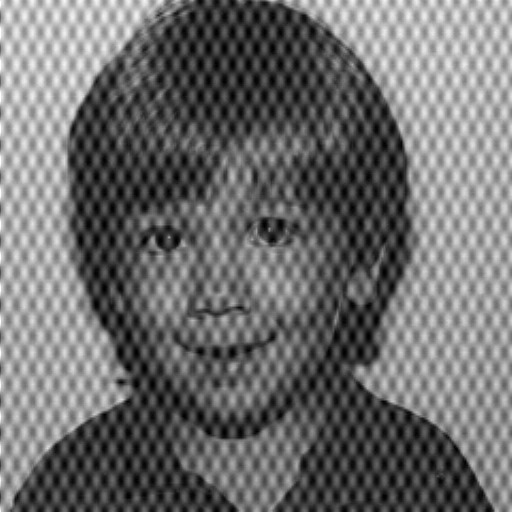
\includegraphics[width=146pt]{../images/boy_noisy}
  }
  \subfigure[FFT]{
    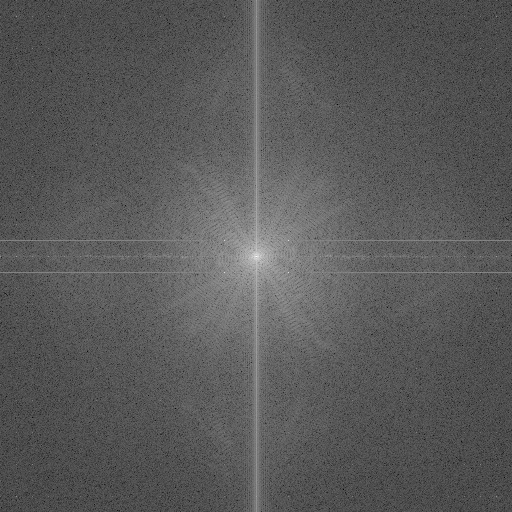
\includegraphics[width=146pt]{../images/boy_noisy_fft_orig}
  }
  \subfigure[Corrected FFT]{
    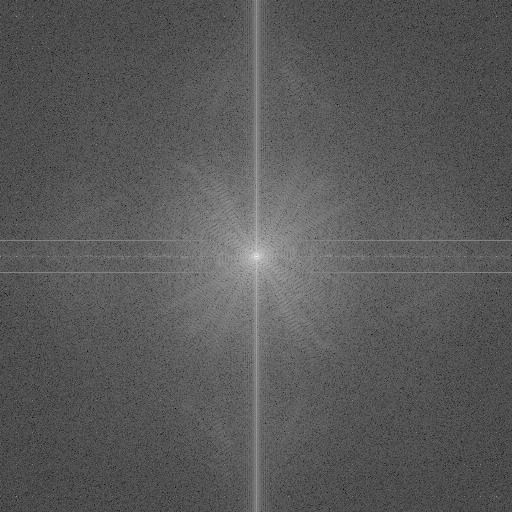
\includegraphics[width=146pt]{../images/boy_noisy_fft_fixed}
  }
  \subfigure[Corrected Image]{
    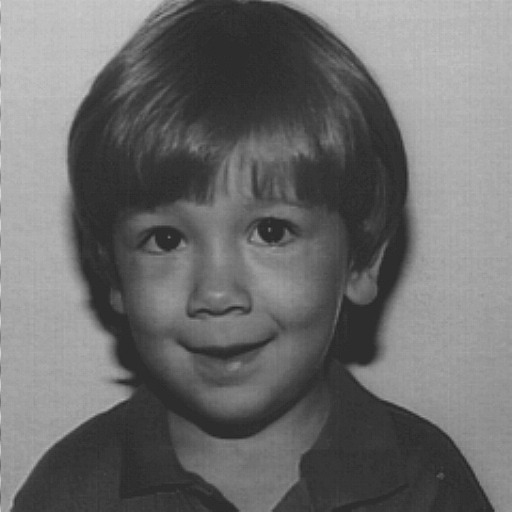
\includegraphics[width=146pt]{../images/boy_noisy_fixed}
  }
  \subfigure[FFT Zoomed]{
    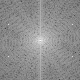
\includegraphics[width=146pt]{../images/boy_noisy_fft_orig_zoomed}
  }
  \subfigure[Corrected FFT Zoomed]{
    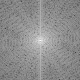
\includegraphics[width=146pt]{../images/boy_noisy_fft_fixed_zoomed}
  }
  \caption{Noisy Image corrected in frequency domain.}
\end{figure}

%\vspace*{\fill}

\begin{figure}[hbt]
  \centering
  \label{fig:boy_filter}
  \subfigure[Original Image]{
    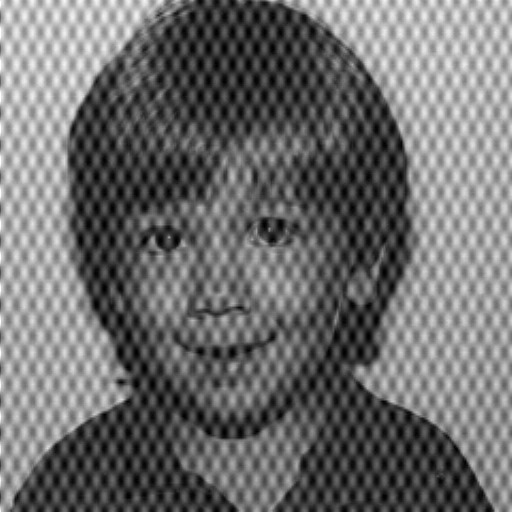
\includegraphics[width=146pt]{../images/boy_noisy}
  }
  \subfigure[5x5]{
    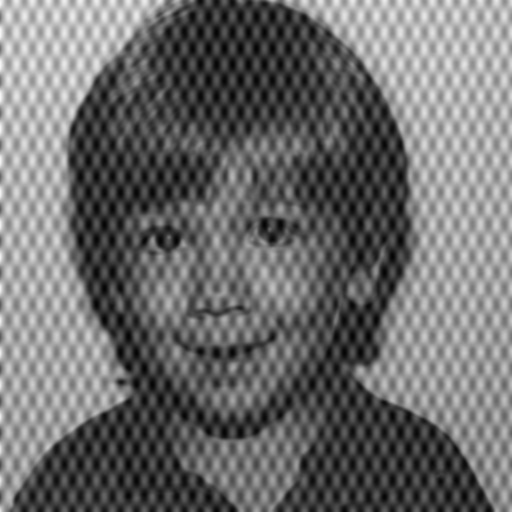
\includegraphics[width=146pt]{../images/boy_noisy_5x5_gaussian}
  }
  \subfigure[7x7]{
    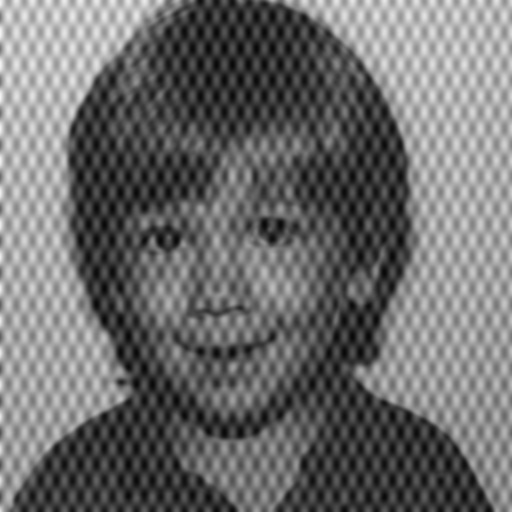
\includegraphics[width=146pt]{../images/boy_noisy_7x7_gaussian}
  }
  \subfigure[15x15]{
    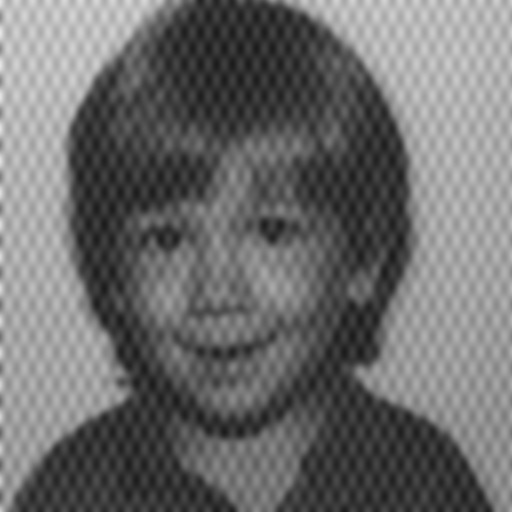
\includegraphics[width=146pt]{../images/boy_noisy_15x15_gaussian}
  }
  \subfigure[25x25]{
    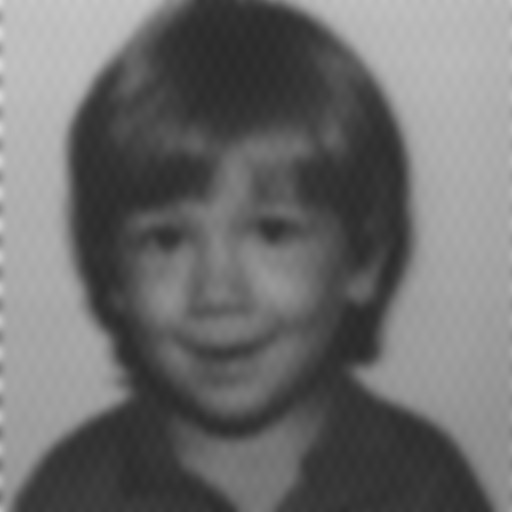
\includegraphics[width=146pt]{../images/boy_noisy_25x25_gaussian}
  }
  \caption{Attempting to remove noise using Gaussian Filters.}
\end{figure}
